\chapter{Модульное тестирование}

\textbf{Цель} модульного тестирования - изолировать отдельные части программы и показать, что по отдельности эти части работоспособны.
С помощью модульных тестов были протестированы основные компоненты приложения.
Как было указано раннее, в базе данных существует 4 основные сущности - две из которых зависят от первичных ключей двух других таблиц. Поэтому было решено провести модульное тестирование двух независимых сущностей. Для каждой сущности существует класс для выполнение определенных действий с указанной сущностью. 
\section{Модуль GroupActions}

\begin{table} 
	\caption{\label{tab:maintable}Тестирование модуля GroupActions}
	\begin{center}
		\begin{tabular}{|l|p{10cm}|}
			\hline
			\multicolumn{2}{|c|}{Проверка наличия группы с название group1} \\
			\hline
			Входные данные & \{groupid1: 104, groupid2:105, groupname1:group1, groupname2:group2\} \\
			Ожидаемый результат &  \\ True
			Задействовано методов класса & 2(InsertGroup, ContainsGroup)\\
			\hline
			\multicolumn{2}{|c|}{Проверка отсутствия группы с название nogroup} \\
			\hline
			Входные данные & \{groupid1: 104, groupid2:105, groupname1:group1, groupname2:group2\} \\
			Ожидаемый результат &  \\ False
			Задействовано методов класса & 2(InsertGroup, ContainsGroup)\\
			\hline
			\multicolumn{2}{|c|}{Нахождение группы по id: 999} \\
			\hline
			Входные данные & \{groupid: 999,groupname:group1,\} \\
			Ожидаемый результат &  \\ True
			Задействовано методов класса & 2(InsertGroup, FindGroupById)\\
			\hline
			\multicolumn{2}{|c|}{Нахождение группы по groupname: group1} \\
			\hline
			Входные данные & \{groupid: 999,groupname:group1,\} \\
			Ожидаемый результат &  \\ True
			Задействовано методов класса & 2(InsertGroup, FindGroupByName)\\
			\hline
			\multicolumn{2}{|c|}{\textbf{Mock тест}: Удаления группы из таблицы Group} \\
			\hline
			Входные данные & 3 объекта класса User с groupid и groupname. idtodelete для удаления \\
			Ожидаемый результат &   Количество объектов в таблице: 2 Сработано сохранений изменений в таблице: 1 \\
			Задействовано методов класса & 1(DeleteGroup)\\
			\hline
			

		\end{tabular}
	\end{center}
\end{table} 


\newpage
\section{Модуль UserActions}
\begin{table} 
	\caption{\label{tab:maintable}Тестирование модуля UserActions}
	\begin{center}
		\begin{tabular}{|l|p{10cm}|}
			\hline
			\multicolumn{2}{|c|}{\textbf{Mock тест}: Вывод пользователей из таблицы User} \\
			\hline
			Входные данные & 3 объекта класса User с userid и usercity \\
			Ожидаемый результат &  Вывод списка с 3-мя объектами класса User \\
			Задействовано методов класса & 1(SelectAllUsers) \\
			\hline
			\multicolumn{2}{|c|}{\textbf{Mock тест}: Добавление пользователя в таблицу User} \\
			\hline
			Входные данные & 3 объекта класса User с userid и usercity\\
			Ожидаемый результат &   Сработано добавлений в таблицу: 1 Сработано сохранений изменений в таблице: 1 \\
			Задействовано методов класса & 1(InsertUser)\\
			\hline
			\multicolumn{2}{|c|}{\textbf{Mock тест}: Нахождение пользователя по userid в таблице User} \\
			\hline
			Входные данные & 3 объекта класса User с userid и usercity. findid для поиска\\
			Ожидаемый результат & Результат метода не NULL \\
			Задействовано методов класса & 1(FindUser)\\
			\hline
			
			\multicolumn{2}{|c|}{\textbf{Mock тест}: Изменение  города пользователя в таблице User} \\
			\hline
			Входные данные & 3 объекта класса User с userid и usercity. newcity для обновления города второго пользователя\\
			Ожидаемый результат &  значение newcity равен городу usercity второго пользователя\\
			Задействовано методов класса & 1(UpdateUser,SelectAllUsers для представления таблицы в виде списка))\\
			\hline
		\end{tabular}
	\end{center}
\end{table} 

\newpage
\section{Модуль KudaGoApi}

Данный модуль отправляет POST-запрос для получения актуальной информации о концертах группы, которую мы указываем в параметрах POST-запроса.
Не смотря на то, что данный API активно используется в приложении, протестировать его крайне сложно, т.к. его результаты зависят от происходящих концертах в реальной жизни, следовательно результаты тестов не постоянны. Но были протестированы 2 простых случая, в которых проверяется результат при попытки получить информацию о ближайших концертах с пустым и null именем. 
\begin{table} 
	\caption{\label{tab:maintable}Тестирование модуля KudaGoApi}
		\begin{tabular}{|l|p{10cm}|}
\hline
\multicolumn{2}{|c|}{Проверка наличия концерта группы ''} \\
\hline
Входные данные & \{groupname = String.Empty\} \\
Ожидаемый результат &   null \\
Задействовано методов класса & 1(GetAllConcertsByGroup)\\
\hline
\multicolumn{2}{|c|}{Проверка наличия концерта группы ''} \\
\hline
Входные данные & \{groupname = null\} \\
Ожидаемый результат &   null \\
Задействовано методов класса & 1(GetAllConcertsByGroup)\\
\hline
		\end{tabular}
\end{table} 

\section{Покрытие}
\begin{figure}
	\centering
	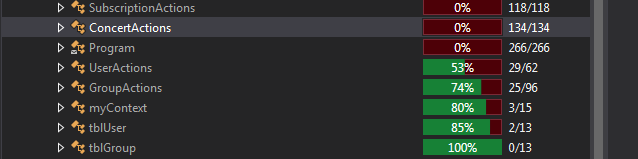
\includegraphics[scale=1]{CoverUnit.PNG}
	\caption{Покрытие после модульных тестов, включая Mock-тесты }
	\label{image:cover-unit}
\end{figure}
